\documentclass[a4paper,11pt]{article}
\usepackage{graphicx}
\usepackage{wrapfig}
\usepackage[a4paper, inner=3cm, outer=3cm, top=3cm, bottom=3cm, offset=0cm]{geometry}
\author{Kenneth Cross}
\title{\textbf{Scheduling Algorithm}}
\date{\today}

\begin{document}
\pagenumbering{gobble}
\maketitle
\newpage
\tableofcontents
\newpage
\pagenumbering{arabic}
\setcounter{page}{1}

\newpage

\section{Methodology}

1) Staff Generation: Stored in a possibility matrix
2) Staff Optimization
3) Schedule Based on Staff Optimization Sum
4) Schedule Satisfaction Optimization

Maximization Factors
* Localization: establish potential rhythms and patterns for objects
* Position Preference: establish staff shift preferences
* Employee Preference: establish a hierarchy of skill based labor and give preference of desirable shifts to skilled employees. 

Multiple Shift Additions: Morning, Afternoon, Graveyard aka MAG

\begin{wrapfigure}{r}{4.5cm}
    \includegraphics[height=10cm]{graph.eps}
    \caption{\small Algorithm Digraph}
\end{wrapfigure}

\section{Modules and Functions}

The entire depth of the inner workings of the program/algorithm are outlined here. 
The subsections try to follow a logical working order of pragmatic flow.

\subsection{Roster Initializations}
\subsection{Workday Validation}
\subsection{Rostering Optimizations}

There are currently four values considered for the final roster optimizer value.
The day difficulty, outstanding employee, position preference, and the employee day preference values and their relationship are what determine the optimizer value.
Any undesirable relationships and traits are given zero points or subtract points, as optimizer values can be negative.
Day preferences are given on the availability grid with a value of zero through five, where zero indicates the impossibility of work and five is the most highly desired day to work.
The position preference value currently only determines the preference of one position, and it is a number, the position index to which they prefer.
The other two values are boolean, which is easy to sum.

All positive relationships and values are given one point and summed, except all the points on day preferences are added instead of a single point.

The relationships needed to accrue points are the following:
1) Outstanding employee and difficult day
2) Difficult day with no outstanding employee in preferred position, then a point is subtracted.

The entire roster is sorted from highest to lowest by optimizer value then given to the scheduler function.

\subsection{Scheduler Optimizations}
\subsection{Multi-Shift Support}

This should be taken care of in the scheduler algorithm rather than the rostering algorithm.
This makes sense because rostering will calculate all possibilities of a person's availability rather than overlook other possibilities for other shifts.
The scheduler should have a section to combine and compare full shift schedules where logic should be performed for optimizations and shifting conflicts or other legal parameters.

\subsection{Multi-Shift Optimizations}

\section{Data Representations}

Incoming input is currently contained in two separate CSV files. 
One file contains employee availability where the position section is a preference as to how many times per week someone would like to perform that position. The other file contains what types of positions are required and how many of each for every day of the week.


\end{document}
